
\chapter{Additional Links}\label{ch:links}

\noindent All code and latex-files used in this document are included in the Github repository linked below.

\subsection*{Github repository link}

\begin{itemize}
    \item \url{https://github.com/Ola-R-R/Master-Thesis}
\end{itemize} 

\ \\

\noindent The data collected from Norges Bank is from the website linked below.

\subsection*{Norges Bank link}

\begin{itemize}
    \item \url{https://www.norges-bank.no/en/topics/Statistics/norwegian-government-securities/zero-coupon-yields/}
\end{itemize}

\chapter{Additional Figures}

\begin{figure}[!htbp]
    \centering
    \captionsetup{type=figure}
    \begin{subfigure}{0.49\textwidth}
        \centering
        \captionsetup{justification=centering}
        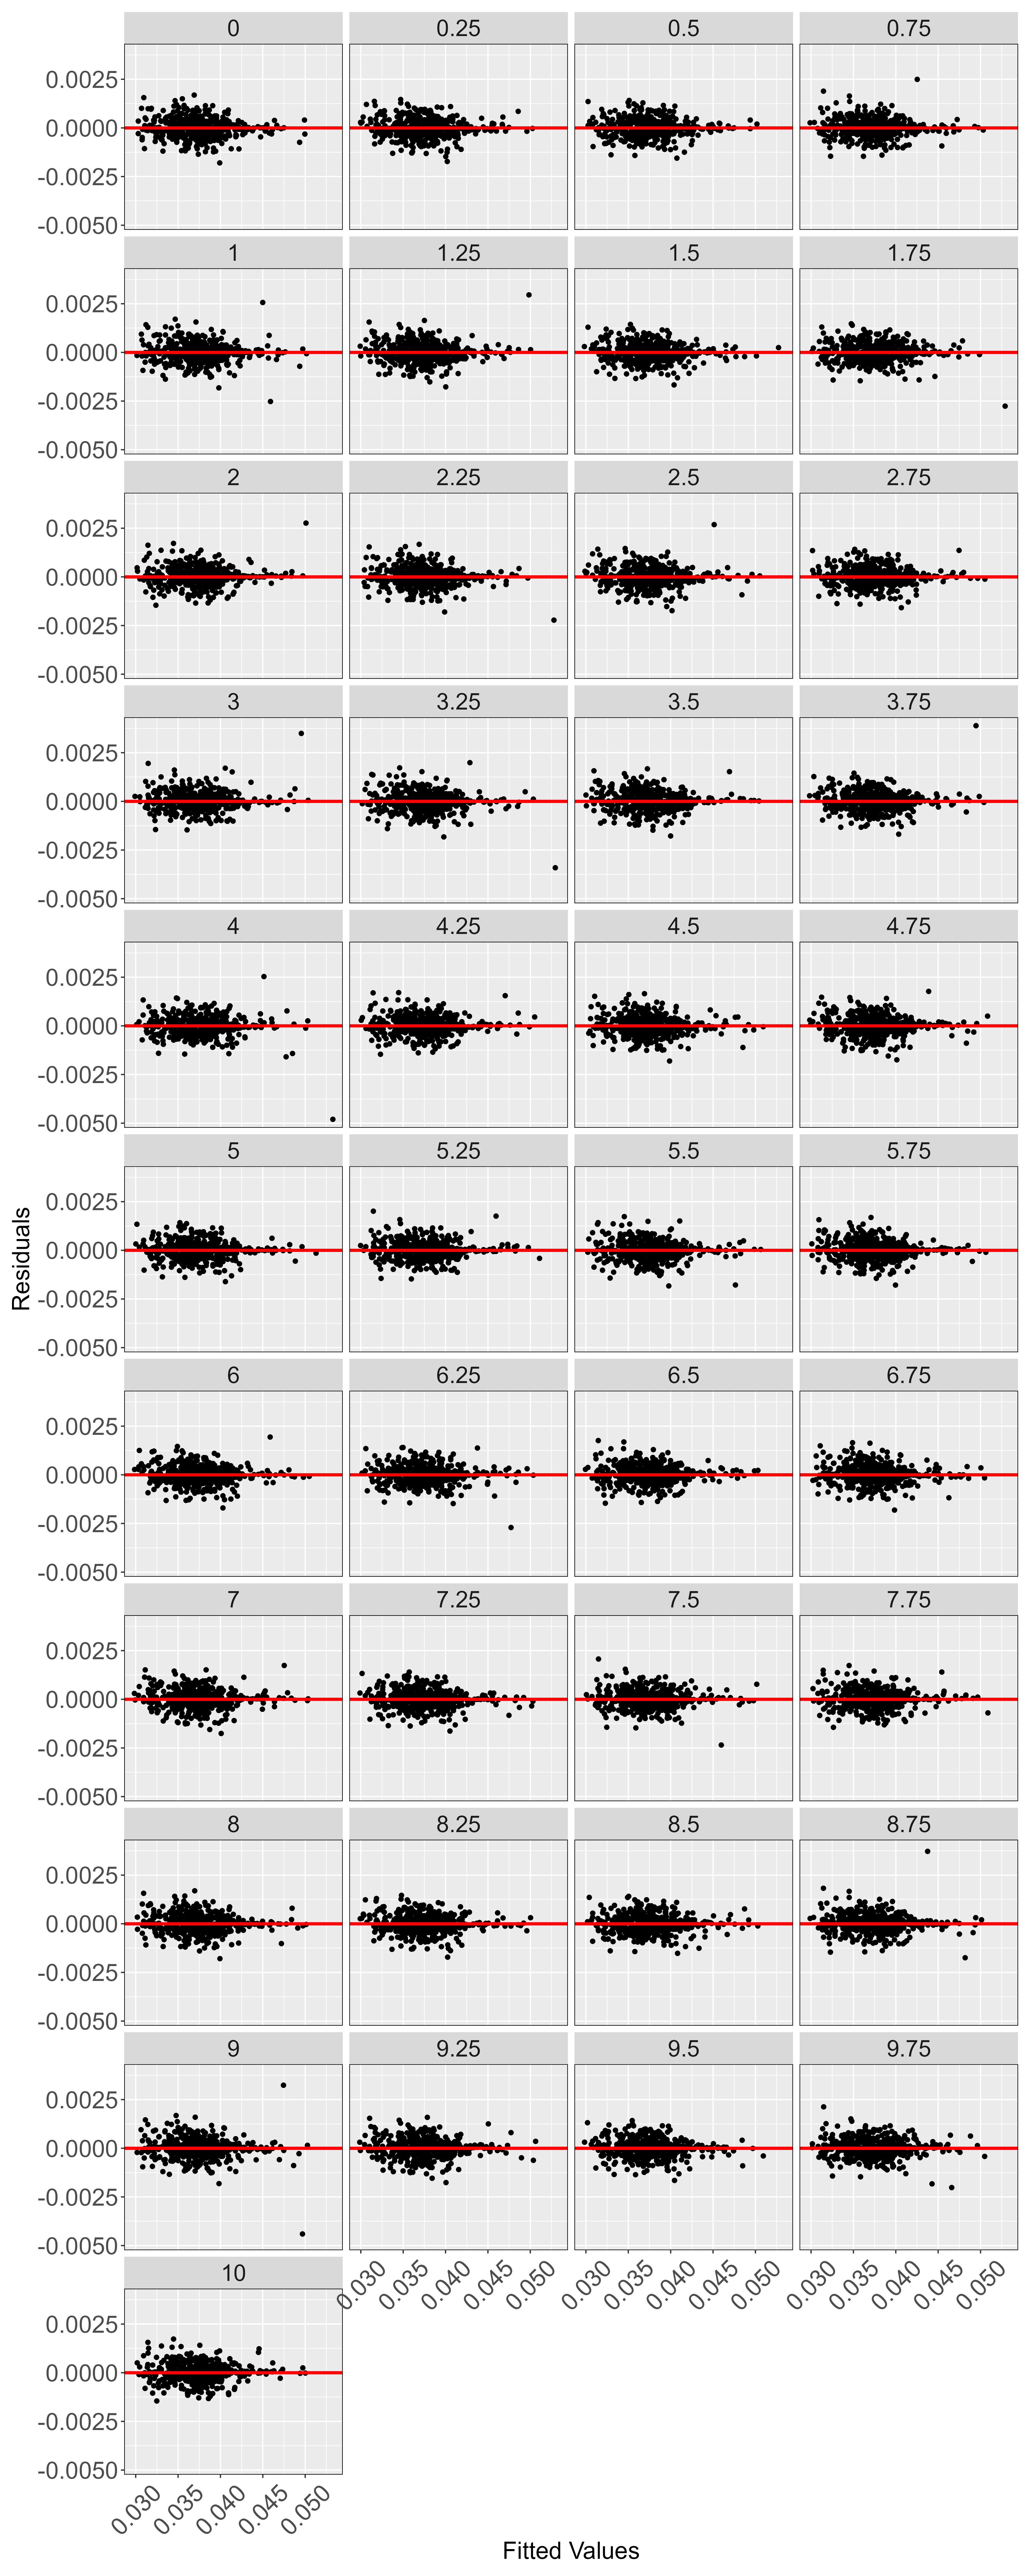
\includegraphics[width=\textwidth]{Figures/Model Checking/zero_coupon_yields_phase_3_HJM_2F_procedure_2_poly_model_fitted_vs_residual_plot.png}
        \subcaption{Volatilities fitted using polynomials.}
        \label{fig:resid vs fit poly model p 2}
    \end{subfigure}
    \hfill
    \begin{subfigure}{0.49\textwidth}
        \centering
        \captionsetup{justification=centering}
        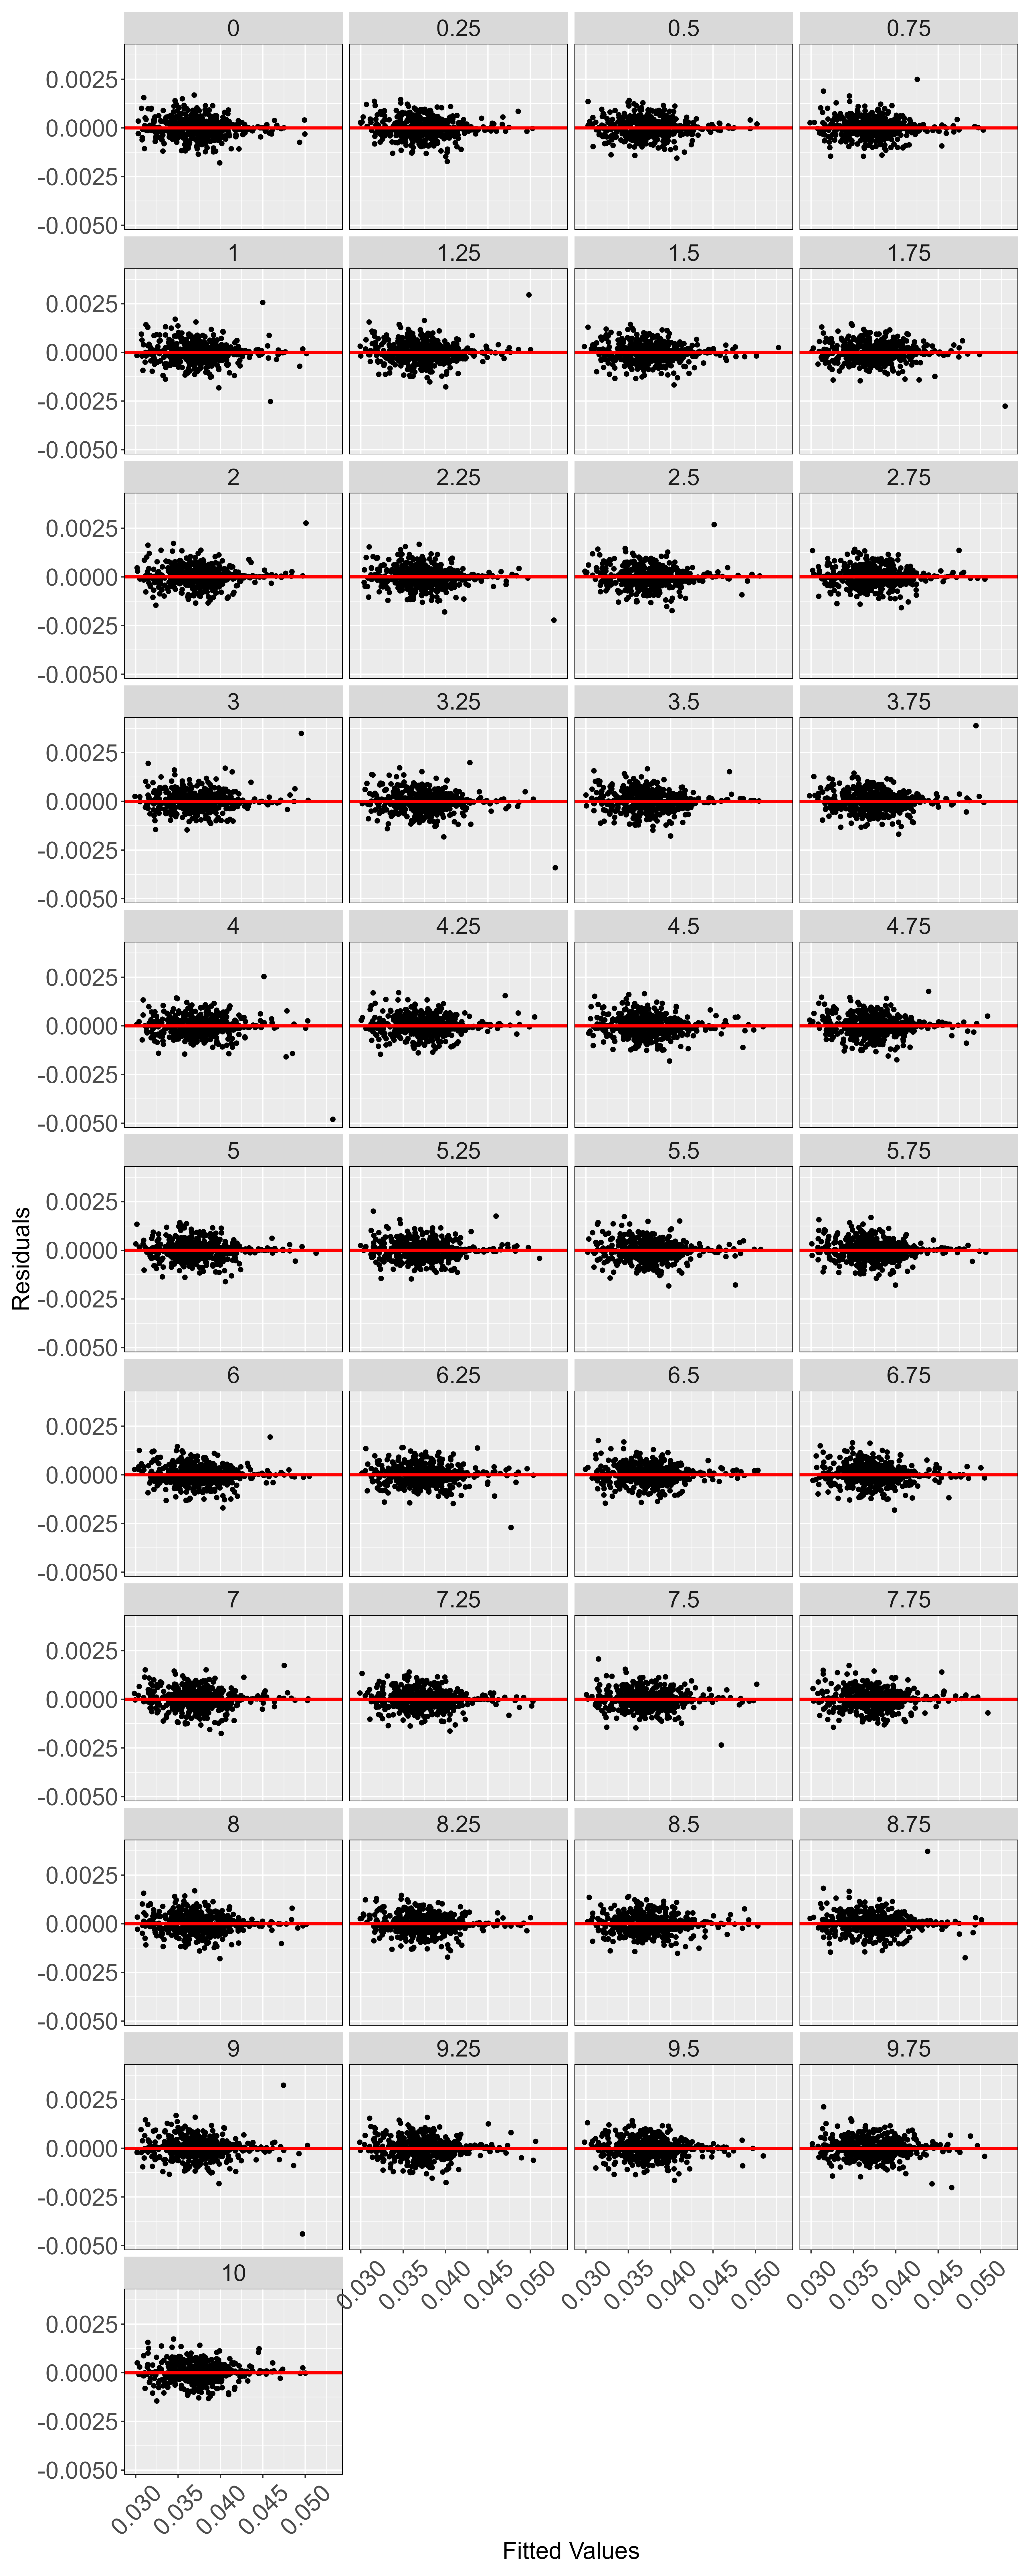
\includegraphics[width=\textwidth]{Figures/Model Checking/zero_coupon_yields_phase_3_HJM_2F_procedure_2_spline_model_fitted_vs_residual_plot.png}
        \subcaption{Volatilities fitted using splines.}
        \label{fig:resid vs fit spline model p 2}
    \end{subfigure}
    \caption[The Residuals vs. Fits Plots for the models using Procedure 2 for all tenors.]{The Residuals vs. Fits Plots for the models using Procedure 2 for all tenors. They show that there is equal variance across all fitted values if we take away the outliers at larger fitted values. There are so few large fitted values, so this doesn't mean that the assumption is wrong.}
    \label{fig:resid vs fit p 2}
\end{figure}

\begin{figure}[!htbp]
    \centering
    \captionsetup{type=figure}
    \begin{subfigure}{0.49\textwidth}
        \centering
        \captionsetup{justification=centering}
        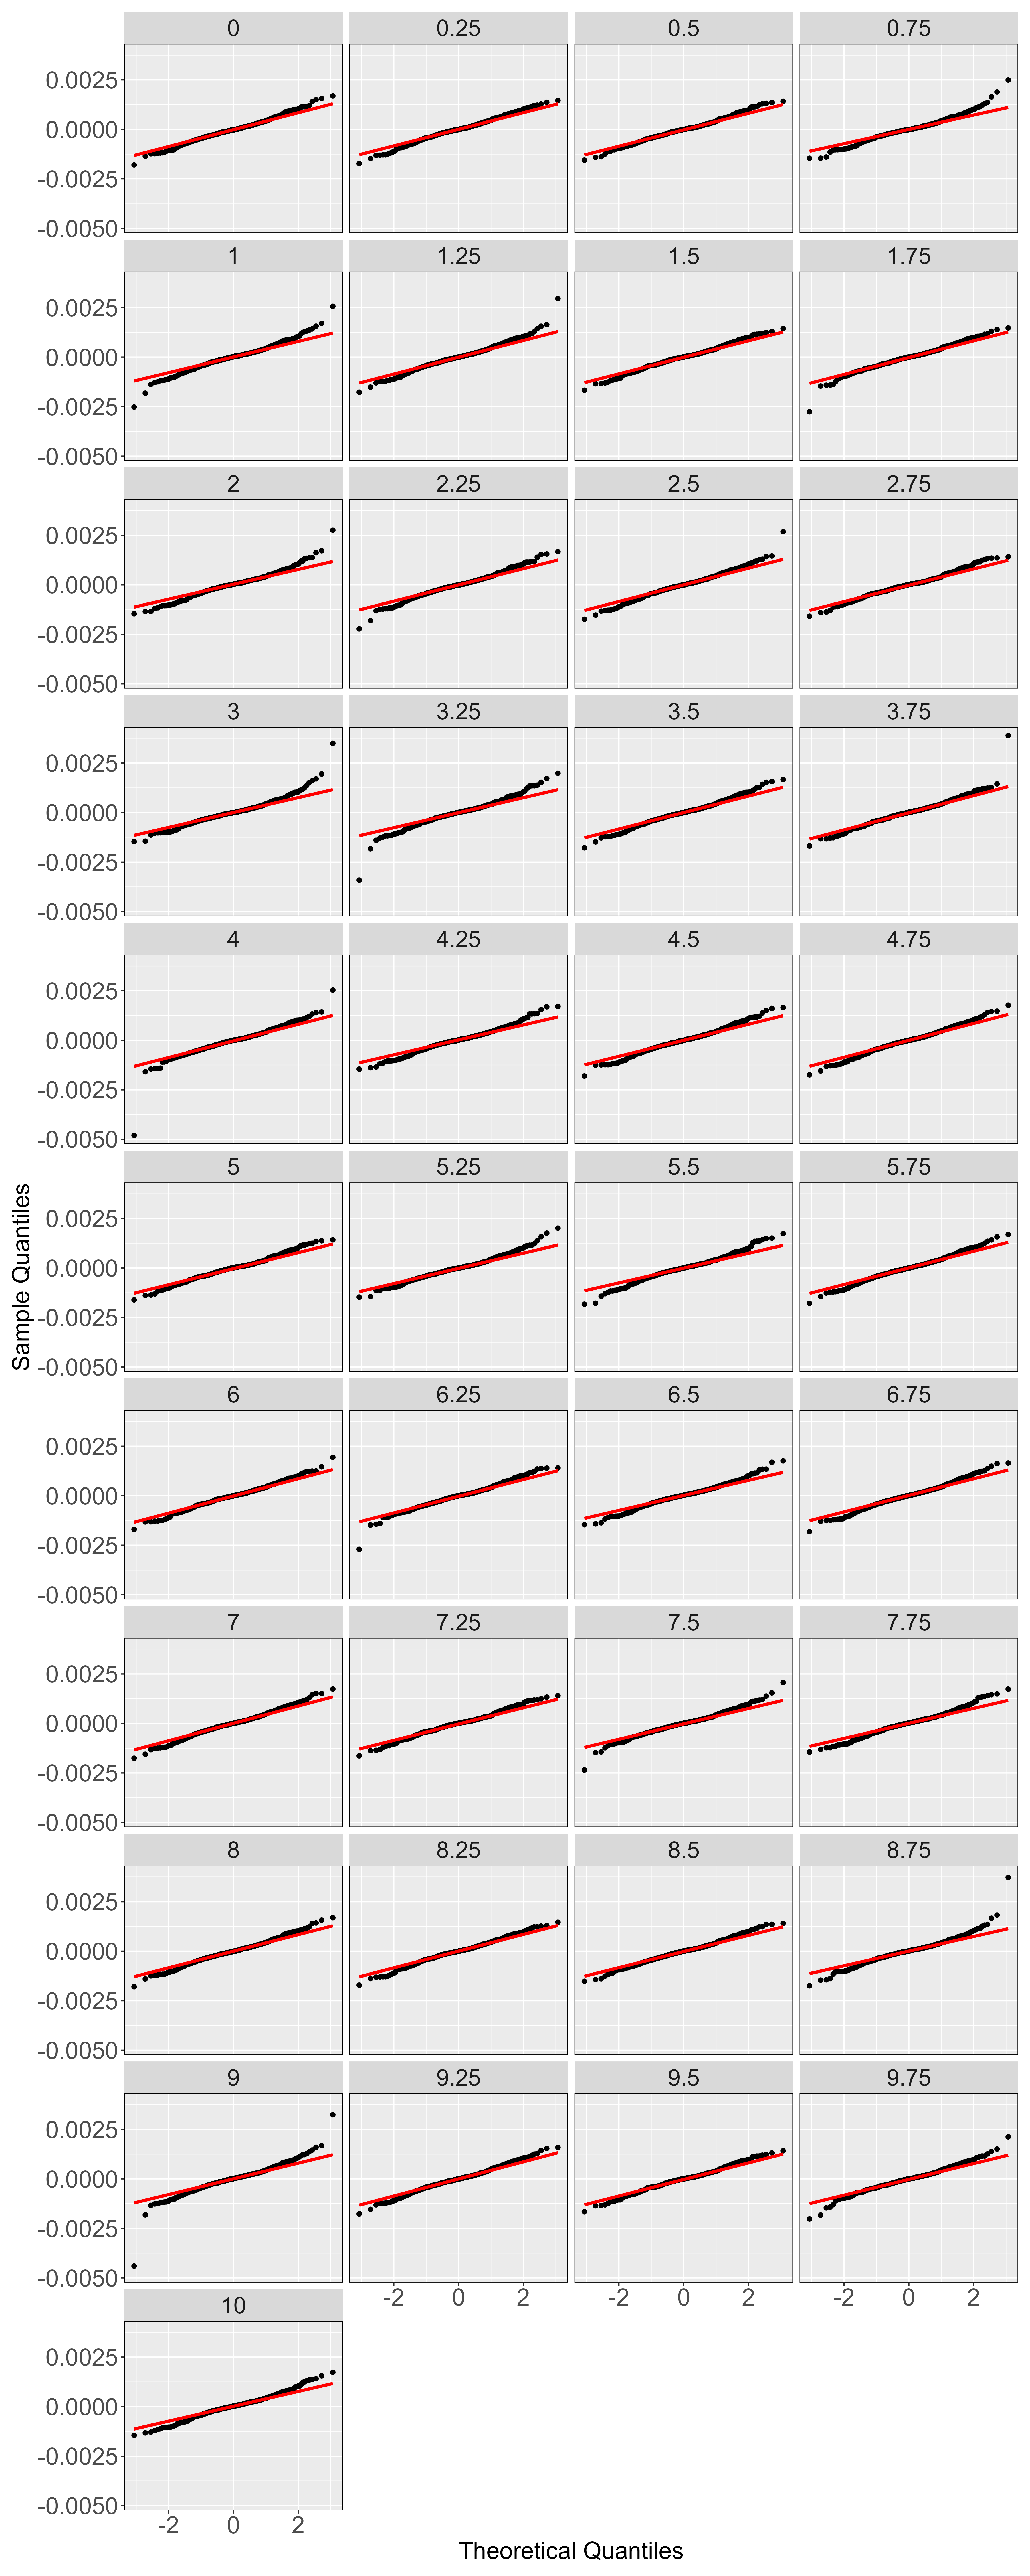
\includegraphics[width=\textwidth]{Figures/Model Checking/zero_coupon_yields_phase_3_HJM_2F_procedure_2_poly_model_qq_plot.png}
        \subcaption{Volatilities fitted using polynomials.}
        \label{fig:qq poly model p 2}
    \end{subfigure}
    \hfill
    \begin{subfigure}{0.49\textwidth}
        \centering
        \captionsetup{justification=centering}
        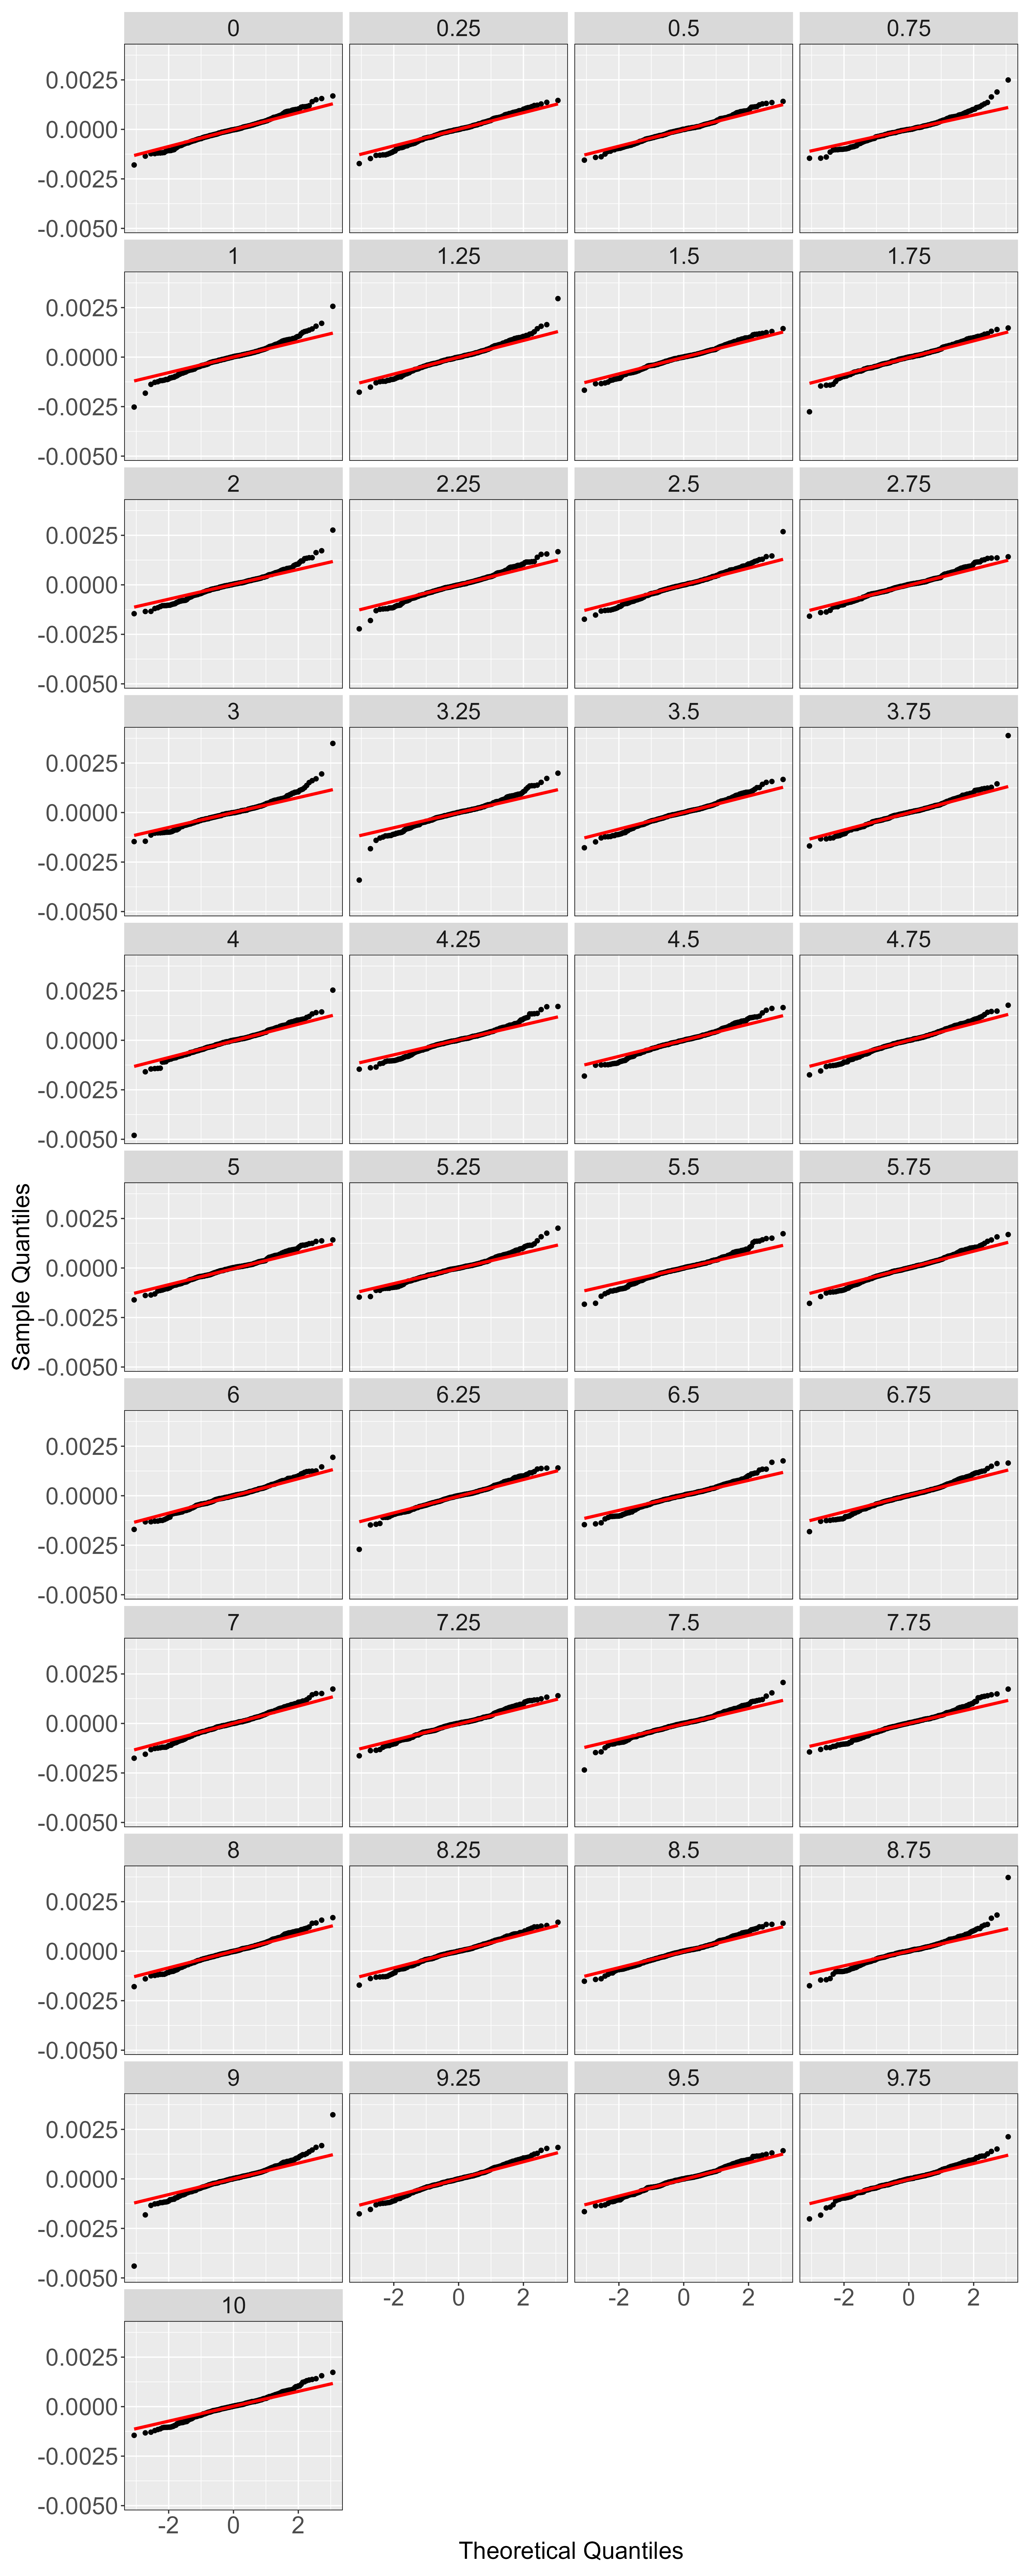
\includegraphics[width=\textwidth]{Figures/Model Checking/zero_coupon_yields_phase_3_HJM_2F_procedure_2_spline_model_qq_plot.png}
        \subcaption{Volatilities fitted using splines.}
        \label{fig:qq spline model p 2}
    \end{subfigure}
    \caption[The QQ-Plots for the models using Procedure 2 for all tenors.]{The QQ-Plots for the models using Procedure 2 for all tenors. They show that the models can predict the distribution of the real data exactly, although a few tenors have heavier tails.}
    \label{fig:qq p 2}
\end{figure}

